% Copyright (C) 2010,2011,2012 The ESPResSo project
% Copyright (C) 2002,2003,2004,2005,2006,2007,2008,2009,2010 
%    Max-Planck-Institute for Polymer Research, Theory Group
%  
% This file is part of ESPResSo.
%   
% ESPResSo is free software: you can redistribute it and/or modify it
% under the terms of the GNU General Public License as published by the
% Free Software Foundation, either version 3 of the License, or (at your
% option) any later version.
%  
% ESPResSo is distributed in the hope that it will be useful, but
% WITHOUT ANY WARRANTY; without even the implied warranty of
% MERCHANTABILITY or FITNESS FOR A PARTICULAR PURPOSE.  See the GNU
% General Public License for more details.
%  
% You should have received a copy of the GNU General Public License
% along with this program.  If not, see <http://www.gnu.org/licenses/>.
%
\newcommand{\taumax}{\tau_{\mathrm{max}}}
\newcommand{\taumin}{\tau_{\mathrm{min}}}
\chapter{Analysis}
\label{chap:analysis}
\index{analysis}
\newescommand{analyze}

\es provides some tools for online (during the simulation run) and
offline (on stored data) analysis of your simulation. The
\keyword{analyze} command has two main uses: Calculation of
observables (\keyword{analyze \var{observable}}) and definition and
analysis of topologies in the system (\keyword{analyze \var{topology
    command}}).

In addition, \es offers the command \keyword{uwerr} (see section
\ref{sec:uwerr} for computing statistical errors in time series.

\section{Measuring observables}

The command \keyword{analyze} provides online-calculation of local and
global observables. 

\subsection{Minimal distances between particles}
\label{analyze:mindist}
\label{analyze:distto}
\analyzeindex{minimal particle distance}
\analyzeindex{particle distance}

\begin{essyntax}
  \variant{1} analyze mindist \opt{\var{type\_list\_a} \var{type\_list\_b}}
  \variant{2} analyze distto \var{pid}
  \variant{3} analyze distto \var{x} \var{y} \var{z}
\end{essyntax}

Variant \variant{1} returns the minimal distance between two particles
in the system. If the type-lists are given, then the minimal distance
between particles of only those types is determined.

\keyword{distto} returns the minimal distance of all particles to
particle \var{pid} (variant \variant{2}), or to the coordinates
(\var{x}, \var{y}, \var{z}) (Variant \variant{3}).

\subsection{Particles in the neighbourhood}
\label{analyze:nbhood}
\analyzeindex{particles in the neighbourhood}

\begin{essyntax}
 \variant{1} analyze nbhood \var{pid} \var{r\_catch}
 \variant{2} analyze nbhood \var{x} \var{y} \var{z}
 \var{r_catch}
\end{essyntax}
Returns a Tcl-list of the particle ids of all particles within a given
radius \var{r\_catch} around the position of the particle with number
\var{pid} in variant \variant{1} or around the spatial coordinate
(\var{x}, \var{y}, \var{z}) in variant \variant{2}.

\subsection{Particle distribution}
\label{analyze:distribution}
\analyzeindex{particle distribution}

\begin{essyntax}
  analyze distribution \var{part\_type\_list\_a} \var{part\_type\_list\_b}
  \opt{\var{rmin} \opt{\var{rmax} \opt{\var{rbins} 
        \opt{\var{log\_flag} \opt{\var{int\_flag}}}}}}
\end{essyntax}
Returns its parameters and the distance distribution of particles with
types specified in \var{part\_type\_list\_a} around particles with
types specified in \var{part\_type\_list\_b} with distances between
\var{rmin} and \var{rmax}, binned into \var{rbins} bins. The
bins are either equidistant (if $\var{log\_flag} = 0$) or
logarithmically equidistant (if $\var{log\_flag} \geq 1$). If an
integrated distribution is required, use $\var{int\_flag}=1$. The
distance is defined as the \emph{minimal} distance between a particle
of one group to any of the other group.

\minisec{Output format} 

The output corresponds to the blockfile format (see section
\vref{sec:structured-file-format}):
\begin{code}
\{ \var{parameters} \} 
\{ 
  \{ \var{r} \var{dist(r)} \} 
  \vdots 
\}
\end{code}

\subsection{Radial density map}
\label{analyze:radialdensitymap}

\begin{essyntax}
  analyze radial_density_map \var{xbins} \var{ybins} \var{xrange} \var{yrange}
  \opt{\var{axisofrotation} \var{centerofrotation} \var{beadtypelist}
  \opt{\var{thetabins}}}
\end{essyntax}

Returns the radial density of particles around a given
axis. Parameters are:

\todo{Someone who knows or wrote this command should check this.}

\begin{itemize}
\item \var{xbins} histogram bins in x direction.
\item \var{ybins} histogram bins in y direction.
\item \var{xrange} range for analysis in x direction.
\item \var{yrange} range for analysis in y direction.
\item \var{axisofrotation} rotate around given axis. (x, y, or z)
\item \var{centerofrotation} rotate around given point.
\item \var{beadtypelist} only analyze beads of given types.
\item \var{thetabins} histogram bins in angle theta.
\end{itemize}

\subsection{Modes}
\label{analyze:modes2d}

\begin{essyntax}
  analyze modes2d
\end{essyntax}

Analyzes the modes of a configuration. Requires that a grid is set and
that the system contains more than two particles. Output are four
numbers in the order:

\begin{displaymath}
ht_{RE}\qquad ht_{IM}\qquad \theta_{RE}\qquad \theta_{IM}
\end{displaymath}

\subsection{Lipid orientation}
\label{analyze:lipids}

\begin{essyntax}
  \variant{1} analyze get_lipid_orients
  \variant{2} analyze lipid_orient_order
\end{essyntax}

\todo{Document the usage!}

\subsection{Bilayers}
\label{analyze:bilayers}

\begin{essyntax}
  \variant{1} analyze bilayer_set
  \variant{2} analyze bilayer_density_profile
\end{essyntax}

\todo{Document the usage!}

\subsection{GPB}
\label{analyze:cellgpb}

\begin{essyntax}
  analyze cell_gpb \var{Manning parameter} \var{outer cell radius}
  \var{inner cell radius} \opt{\var{accuracy}
    \opt{\var{number of interactions}}}
\end{essyntax}

\todo{Document the usage and what it is!}

\subsection{Get folded positions}
\label{analyze:folded}

\begin{essyntax}
  analyze get_folded_positions \opt{-molecule} \opt{shift \var{x} \var{y} \var{z}}
\end{essyntax}

Outputs the folded positions of particles. Without any parameters, the
positions of all particles are given, folded to the box length. The
optional parameter \keyword{-molecule} ensures that molecules
(particle groups) are kept intact. The optional shift parameters can
be used to shift the not separated molecules if needed.

\subsection{Vkappa}
\label{analyze:Vkappa}

\begin{essyntax}
  analyze Vkappa \opt{\alt{ reset \asep read \asep set \var{V_{\kappa, 1}} \var{V_{\kappa, 2}} \var{avk} } }
\end{essyntax}

\todo{Document the usage and what it is!}

\subsection{Radial distribution function}
\label{analyze:rdf}
\label{analyze:<rdf>}
\analyzeindex{radial distribution function $g(r)$}

\begin{essyntax}
  analyze \alt{rdf \asep <rdf>} 
  \var{part\_type\_list\_a} \var{part\_type\_list\_b} 
  \opt{\var{rmin} \var{rmax} \var{rbins}}
\end{essyntax}
Returns its parameters and the radial distribution function (rdf) of
particles with types specified in \var{part\_type\_list\_a} around
particles with types specified in \var{part\_type\_list\_b}. The range
is given by \var{rmin} and \var{rmax} and is divided into
\var{rbins} equidistant bins.

\minisec{Output format}

The output corresponds to the blockfile format (see section
\vref{sec:structured-file-format}):
\begin{code}
\{ \var{parameters} \} 
\{ 
  \{ \var{r} \var{rdf(r)} \} 
  \vdots
\}
\end{code}

\subsection{Structure factor}
\label{analyze:structurefactor}
\analyzeindex{structure factor $S(q)$}

\begin{essyntax}
  analyze structurefactor \var{type} \var{order}
\end{essyntax}

Returns the spherically averaged structure factor $S(q)$ for particles
of a given type \var{type}. The $S(q)$ is calculated for all possible
wave vectors, $\frac{2\pi}{L} <= q <= \frac{2\pi}{L}\var{order}$. Do
not chose parameter \var{order} too large, because the number of
calculations grows as $\var{order}^3$. 


\minisec{Output format} 

The output corresponds to the blockfile format (see section
\vref{sec:structured-file-format}):
\begin{code}
\{ \var{q\_value} \var{S(q)\_value} \} 
\vdots
\end{code}

\subsection{Van-Hove autocorrelation function $G(r,t)$}
\label{analyze:vanhove}
\analyzeindex{van Hove autocorrelation function $G(r,t)$}
\begin{essyntax}
  analyze vanhove \var{type} \var{rmin} \var{rmax} \var{rbins}
  \opt{\var{tmax}}
\end{essyntax}
Returns the van Hove auto correlation function $G(r,t)$ and the mean
square displacement $msd(t)$ for particles of type \var{ptype} for the
configurations stored in the array configs. This tool assumes that the
configurations stored with \codebox{analyze append} (see section
\vref{sec:stored-configs}) are stored at equidistant time intervals.
$G(r,t)$ is calculated for each multiple of this time intervals. For
each time t the distribution of particle displacements is calculated
according to the specification given by \var{rmin}, \var{rmax} and
\var{rbins}. Optional argument \var{tmax} defines the maximum value
of $t$ for which $G(r,t)$ is calculated. If it is omitted or set to
zero, maximum possible value is used.
If the particles perform a random walk (\ie a normal
diffusion process) $G(r,t)/r^2$ is a Gaussian distribution for all
times.  Deviations of this behavior hint on another diffusion process
or on the fact that your system has not reached the diffusive regime.
In this case it is also very questionable to calculate a diffusion
constant from the mean square displacement via the Stokes-Einstein
relation. 

\minisec{Output format}
The output corresponds to the blockfile format (see section
\vref{sec:structured-file-format}):
\begin{code}
\{ msd \{ \var{msd(0)} \var{msd(1)} \dots \} \} 
\{ vanhove \{ \{ \var{G(0,0)} \var{G(1,0)} \dots \} 
            \{ \var{G(0,1)} \var{G(1,1)} \dots \}
\vdots
          \}
\}
\end{code}

The $G(r,t)$ are normalized such that the integral over space always
yields $1$.

\subsection{Center of mass}
\label{analyze:centermass}
\analyzeindex{center of mass}
\begin{essyntax}
  analyze centermass \var{part_type}
\end{essyntax}
Returns the center of mass of particles of the given type.

\subsection{Moment of inertia matrix}
\label{analyze:momentofinteratiamatrix}
\label{analyze:find-principal-axis}
\analyzeindex{moment of inertia matrix}
\analyzeindex{principal axis of the moment of inertia}

\begin{essyntax}
  \variant{1} analyze momentofinertiamatrix { \var{typeid} } 
  \variant{2} analyze find_principal_axis \var{typeid}
\end{essyntax}
Variant \variant{1} returns the moment of inertia matrix for particles
of given type \var{typeid}. The output is a list of all the elements
of the 3x3 matrix. Variant \variant{2} returns the eigenvalues and
eigenvectors of the matrix.

\subsection{Gyration tensor}
\label{analyze:gyration-tensor}
\analyzeindex{gyration tensor}

\begin{essyntax}
  analyze gyration\_tensor \opt{\var{typeid}} 
\end{essyntax}
Analyze the gyration tensor of particles of a given type \var{typeid},
or of all particles in the system if no type is given.
Returns a Tcl-list containing the squared radius of gyration,
 three shape descriptors (asphericity, acylindricity,
 and relative shape anisotropy), eigenvalues of the gyration tensor and their
corresponding eigenvectors. The eigenvalues are sorted in descending order.

\subsection{Aggregation}
\label{analyze:aggregation}
\analyzeindex{aggregation}

\begin{essyntax}
  analyze aggregation \var{dist\_criteria} \var{s\_mol\_id}
  \var{f\_mol\_id} \opt{\var{min\_contact} \opt{\var{charge\_criteria}}}
\end{essyntax}
Returns the aggregate size distribution for the molecules in the
molecule id range \var{s\_mol\_id} to \var{f\_mol\_id}. If any
monomers in two different molecules are closer than
\var{dist\_criteria} they are considered to be in the same aggregate.
One can use the optional \var{min\_contact} parameter to specify a
minimum number of contacts such that only molecules having at least
\var{min\_contact} contacts will be considered to be in the same
aggregate. The second optional parameter \var{charge\_criteria}
enables one to consider aggregation state of only oppositely charged
particles.

\subsection{Identifying pearl-necklace structures}
\label{analyze:necklace}
\analyzeindex{pearl-necklace structures}

\begin{essyntax}
 analyze necklace \var{pearl\_threshold} \var{back\_dist} \var{space\_dist}
\var{first} \var{length} 
\end{essyntax}
Algorithm for identifying pearl necklace structures for
polyelectrolytes in poor solvent \citep{limbach03a}. The first three
parameters are tuning parameters for the algorithm:
\var{pearl\_treshold} is the minimal number of monomers in a pearl.
\var{back\_dist} is the number of monomers along the chain backbone
which are excluded from the space distance criterion to form clusters.
\var{space\_dist} is the distance between two monomers up to which
they are considered to belong to the same clusters. The three
parameters may be connected by scaling arguments. Make sure that your
results are only weakly dependent on the exact choice of your
parameters. For the algorithm the coordinates stored in partCfg are
used. The chain itself is defined by the identity first of its first
monomer and the chain length length.  Attention: This function is very
specific to the problem and might not give useful results for other
cases with similar structures.

\subsection{Finding holes}
\label{analyze:holes}
\analyzeindex{finding holes}

\begin{essyntax}
  analyze holes \var{typeid_\mathrm{probe}} \var{mesh\_size} 
\end{essyntax}
Function for the calculation of the unoccupied volume (often also
called free volume) in a system. Details can be found in
\citet{schmitz00a}.  It identifies free space in the simulation box
via a mesh based cluster algorithm.  Free space is defined via a probe
particle and its interactions with other particles which have to be
defined through LJ interactions with the other existing particle types
via the inter command before calling this routine. A point of the mesh
is counted as free space if the distance of the point is larger than
LJ_cut+LJ_offset to any particle as defined by the LJ interaction
parameters between the probe particle type and other particle types.\
How to use this function:\ Define interactions between all (or the
ones you are interested in) particle types in your system and a
fictitious particle type.  Practically one uses the van der Waals radius
of the particles plus the size of the probe you want to use as the
Lennard Jones cutoff. The mesh spacing is the box length divided by
the \var{mesh_size}.

\minisec{Output format}
\begin{code}
\{ \var{n\_holes} \var{mean\_hole\_size} \var{max\_hole\_size} \var{free\_volume\_fraction} 
    \{ \var{sizes} \}
    \{ \var{surfaces} \} 
    \{ \var{element\_lists} \} 
\} 
\end{code}

A hole is defined as a continuous cluster of mesh elements that belong
to the unoccupied volume. Since the function is quite rudimentary it
gives back the whole information suitable for further processing on
the script level. \var{sizes} and \var{surfaces} are given in number
of mesh points, which means you have to calculate the actual size via
the corresponding volume or surface elements yourself. The complete
information is given in the element_lists for each hole. The element
numbers give the position of a mesh point in the linear representation
of the 3D grid (coordinates are in the order x, y, z). Attention: the
algorithm assumes a cubic box. Surface results have not been tested.
Requires the feature LENNARD_JONES.  \todo{I think there is still a
  bug in there (Hanjo)}.

\subsection{Energies}
\label{analyze:energy}
\analyzeindex{energies}

\begin{essyntax}
  \variant{1} analyze energy
  \variant{2} analyze energy \alt{total \asep kinetic \asep coulomb \asep magnetic}
  \variant{3} analyze energy bonded \var{bondid}
  \variant{4} analyze energy nonbonded \var{typeid1} \var{typeid2}
\end{essyntax}
\todo{Describe the different energies components returned by the
  different commands!}
Returns the energies of the system. Variant \variant{1} returns all
the contributions to the total energy. Variant \variant{2} returns the
numerical value of the total energy or its kinetic or Coulomb or magnetic
contributions only. Variants \variant{3} and \variant{4} return the
energy contributions of the bonded resp. non-bonded interactions.

\minisec{Output format (variant \variant{1})}
\begin{code}
\{ energy \var{value} \} \{ kinetic \var{value} \} \{ interaction \var{value} \} \dots 
\end{code}


\subsection{Pressure}
\label{analyze:pressure}
\analyzeindex{pressure}

\begin{essyntax}
  \variant{1} analyze pressure
  \variant{2} analyze pressure total
  \variant{3} analyze pressure \alt{totals \asep ideal \asep coulomb
    \asep \\tot_nonbonded_inter \asep tot_nonbonded_intra}
  \variant{4} analyze pressure bonded \var{bondid}
  \variant{5} analyze pressure nonbonded \var{typeid1} \var{typeid2}
  \variant{6} analyze pressure nonbonded_intra \opt{\var{typeid}}
  \variant{7} analyze pressure nonbonded_inter \opt{\var{typeid}}
\end{essyntax}

Computes the pressure and its contributions in the system. Variant
\variant{1} returns all the contributions to the total pressure.
Variant \variant{2} will return the total pressure only.  Variants
\variant{3}, \variant{4} and \variant{5} return the corresponding
contributions to the total pressure.

\warning{Pressure works only with certain interactions and
features. Read in detail before use!}

\todo{Document arguments nb_inter, nb_intra, tot_nb_inter and
  tot_nb_intra}

The pressure is calculated (if there are no electrostatic interactions) by 
\begin{equation}
\label{eq:ptens}
  p = \frac{2E_{kinetic}}{Vf} + \frac{\sum_{j>i} {F_{ij}r_{ij}}}{3V}
\end{equation}
where $f$ is the number of degrees of freedom of each particle, $V$
is the volume of the system, $E_{kinetic}$ is the kinetic energy, $F_{ij}$ the force between
particles i and j, and $r_{ij}$ is the distance between them.  The kinetic energy divided by the
degrees of freedom is
\begin{equation}
\frac{2E_{kinetic}}{f} = \frac{1}{3}\sum_{i} {m_{i}v_{i}^{2}}
\end {equation}
when the ROTATION option is turned off and
\begin{equation}
\frac{2E_{kinetic}}{f} = \frac{1}{6}\sum_{i}{(m_{i}v_{i}^{2} + I_{i}w_{i}^{2})})
\end{equation}
 when the ROTATION option is compiled in.  $I_{i}$ is the moment of inertia of the particle and
 $w_{i}$ is the angular velocity.

Note that Equation~\ref{eq:ptens} can only be applied to pair potentials and central forces.
Description of how contributions from other interactions are calculated is beyond the scope
of this manual. Three body potentials are implemented following the procedure in 
Ref.~\cite{thompson09a}.
A different formula is used to calculate contribution from electrostatic interactions 
in P3M. For electrostatic interactions, the $k$-space contribution is not 
well tested, so use with caution!
\todo{Description of how electrostatic contribution to Pressure is calculated}
Anything outside that is currently not implemented.
Four-body dihedral potentials are not included.
In case of rigid body rotation, virial contribution from torques is not included.
Constraints of any kind are not currently accounted for in the pressure calculations. 
The pressure is no longer correct, e.g., when particles are confined to a plane.

The command is implemented in parallel.

\minisec{Output format (variant \variant{1})}

\begin{code}
\{ \{ pressure \var{total\_pressure} \}
   \{ ideal \var{ideal\_gas\_pressure} \} 
   \{ \{ \var{bond\_type} \var{pressure} \}
      \vdots
   \}
   \{ \{ \var{nonbonded\_type} \var{pressure} \}
      \vdots
   \}
   \{ coulomb \var{pressure} \}
\}
\end{code}
specifying the pressure, the ideal gas pressure, the
contributions from bonded interactions, the contributions from
non-bonded interactions and the electrostatic contributions.


\subsection{Stress Tensor}
\label{analyze:stresstensor}
\analyzeindex{stress tensor}

\begin{essyntax}
  \variant{1} analyze stress_tensor
  \variant{2} analyze stress_tensor total
  \variant{3} analyze stress_tensor \alt{totals \asep ideal \asep coulomb
    \asep \\tot_nonbonded_inter \asep tot_nonbonded_intra}
  \variant{4} analyze stress_tensor bonded \var{bond_type}
  \variant{5} analyze stress_tensor nonbonded \var{typeid1} \var{typeid2}
  \variant{6} analyze stress_tensor nonbonded_intra \opt{\var{typeid}}
  \variant{7} analyze stress_tensor nonbonded_inter \opt{\var{typeid}}
\end{essyntax}

Computes the stress tensor of the system.  The various options are equivalent to those described by
\keyword{analyze pressure} in \vref{analyze:pressure}. It is called a stress tensor but the sign
convention follows that of a pressure tensor.

\warning{Stress tensor works only with certain interactions and features. 
Same restrictions as in the case of Pressure are applicable 
(see scetion~\ref{analyze:pressure}).}

The stress tensor is calculated by 
\begin{equation}
  p^{(kl)} = \frac{\sum_{i} {m_{i}v_{i}^{(k)}v_{i}^{(l)}}}{V} + \frac{\sum_{j>i}{F_{ij}^{(k)}r_{ij}^{(l)}}}{V}
\end{equation}
where the notation is the same as for \keyword{analyze pressure} in \vref{analyze:pressure} and the
superscripts $k$ and $l$ correspond to the components in the tensors and vectors.  Note that the
angular velocities of the particles are not included in the calculation of the stress tensor.  This
means that when the ROTATION option is compiled in the instantaneous pressure calculated with
\keyword{analyze pressure} will be different from the pressure implied by
the stress tensor.  However, the time averages should be in agreement.


The command is implemented in parallel.

\minisec{Output format (variant \variant{1})}

\begin{code}
\{ \{ pressure \var{total\_pressure\_tensor} \}
   \{ ideal \var{ideal\_gas\_pressure\_tensor} \} 
   \{ \{ \var{bond\_type} \var{pressure\_tensor} \}
      \vdots
   \}
   \{ \{ \var{nonbonded\_type} \var{pressure\_tensor} \}
      \vdots
   \}
   \{ coulomb \var{pressure\_tensor} \}
\}
\end{code}
specifying the pressure tensor, the ideal gas pressure tensor, the
contributions from bonded interactions, the contributions from
non-bonded interactions and the electrostatic contributions.

\subsection{Local Stress Tensor}
\label{analyze:localstresstensor}
\analyzeindex{local stress tensor}

\begin{essyntax}
  analyze local_stress_tensor \var{periodic\_x} \var{periodic\_y} \var{periodic\_z} \var{range\_start\_x} \var{range\_start\_y} \var{range\_start\_z} \var{range\_x} \var{range\_y} \var{range\_z}  \var{bins\_x} \var{bins\_y} \var{bins\_z}
\end{essyntax}

Computes local stress tensors in the system.  A cuboid is defined starting at the coordinate
(\var{range\_start\_x},\var{range\_start\_y},\var{range\_start\_z}) and going to the coordinate
(\var{range\_start\_x}+\var{range\_x}, \var{range\_start\_y}+\var{range\_y},
\var{range\_start\_z}+\var{range\_z}).  This cuboid in divided into \var{bins\_x} bins in the x
direction, \var{bins\_y} bins in the y direction and \var{bins\_z} bins in the z direction such that
the total number of bins is \var{bins\_x}*\var{bins\_y}*\var{bins\_z}.  For each of these bins a stress
tensor is calculated using the Irving Kirkwood method.  That is, a given interaction contributes
towards the stress tensor in a bin proportional to the fraction of the line connecting the two
particles that is within the bin.

If the P3M and MMM1D electrostatic methods are used, these
interactions are not included in the local stress tensor.  The DH and
RF methods, in contrast, are included. Concerning bonded interactions 
only two body interactions (FENE, Harmonic) are included (angular and dihedral are not).
For all electrostatic interactions only the real space part is included.

Care should be taken when using constraints of any kind, since these are not accounted for
in the local stress tensor calculations. 

The command is implemented in parallel.

\minisec{Output format (variant \variant{1})}

\begin{code}
\{ \{ LocalStressTensor \}
   \{ \{ \var{x\_bin} \var{y\_bin} \var{z\_bin} \} \{ \var{pressure\_tensor} \} \}
      \vdots
\}
\end{code}
specifying the local pressure tensor in each bin.

\section{Analyze groups of particles (molecules)}
\analyzeindex{topologies}
\label{analyze:set}

The following set of functions is designed to facilitate analysis of molecules. Molecules are expected to be a group of particles
comprising a contiguous range of particle IDs. Each molecule
is a set of consecutively numbered particles and all molecules
are supposed to consist of the same number of particles.
Some functions in this group require that the particles constituting
a molecule are connected into linear chains (particle $n$ is connected
to $n+1$ and so on) while others are applicable to molecules
of whatever topology.

The \lit{analyze set} command defines the structure of the current
system to be used with some of the analysis functions.

\begin{essyntax}
  \variant{1} analyze set chains \opt{\var{chain\_start} \var{n\_chains}
    \var{chain\_length}}
  \variant{2} analyze set topo\_part\_sync
  \variant{3} analyze set
  %\variant{4} analyze set trapmol \var{mol\_id} \var{xpos} \var{ypos} \var{zpos} \var{isrelative} \var{spring\_constant} \var{drag\_constant} coords \var{trapped\_coord\_x} \var{trapped\_coord\_y} \var{trapped\_coord\_z} noforce\_coords \var{noforce\_coord\_x} \var{noforce\_coord\_y} \var{noforce\_coord\_z}
\end{essyntax}

Variant \variant{1} defines a set of \var{n\_chains} chains of equal
length \var{chain\_length} which start with the particle with particle
number \var{chain\_start} and are consecutively numbered (\ie the last
particle in that topology has number $\var{chain\_start} +
\var{n\_chains}*\var{chain\_length} - 1$). 

Variant \variant{2} synchronizes topology and particle data, assigning \var{mol\_id} values to particles.

Variant \variant{3} will return the chains currently stored.

%\todo{Why is setting up a trap implemented via analyze command?}
%Variant \variant{3} sets a trap on a molecule, i.e.\ an external potential acting on it.
%\var{mol\_id} define the molecule ID on which the trap is set, \var{xpos} \var{ypos} \var{zpos} define coordinates of the centre of the trap. \var{isrelative} is an integer specifying if the trap is relative or absolute. (Requires features: MOLFORCES and EXTERNAL\_FORCES).
%\todo{Trapmol documentation still incomplete.}


\subsection{Chains}
\analyzeindex{chains}

All analysis functions in this section require the topology of the
chains to be set correctly.  The topology can be provided upon
calling. This (re-)sets the structure info permanently, \ie it is only
required once.

\subsubsection{End-to-end distance}
\analyzeindex{end-to-end distance of a chain}

\begin{essyntax}
  analyze \alt{re \asep <re>} 
  \opt{\var{chain\_start} \var{n\_chains} \var{chain\_length}}
\end{essyntax}
Returns the quadratic end-to-end-distance and its root averaged over
all chains.  If \lit{<re>} is used, the distance is averaged over all
stored configurations (see section \vref{sec:stored-configs}).

\minisec{Output format}
\begin{code}
\{ \var{re} \var{error\_of\_re} \var{re2} \var{error\_of\_re2} \}
\end{code}

\subsubsection{Radius of gyration}
\analyzeindex{radius of gyration of a chain}

\begin{essyntax}
  analyze \alt{rg \asep <rg>} 
  \opt{\var{chain\_start} \var{n\_chains} \var{chain\_length}}
\end{essyntax}
Returns the radius of gyration averaged over all chains. It is a radius
of a sphere, which would have the same moment of inertia as the molecule, 
defined as
\begin{equation}
\label{eq:Rg}
R_{\mathrm G}^2 = \frac{1}{N} \sum\limits_{i=1}^{N} \left(\vec r_i - \vec r_{\mathrm{cm}}\right)^2\,,
\end{equation}
where $\vec r_i$ are position vectors of individual particles constituting a molecule
and $\vec r_{\mathrm{cm}}$ is the position vector of its centre of mass. The sum runs
over all $N$ particles comprising the molecule. For more information see
any polymer science book, e.g.~\cite{rubinstein03a}.
If \lit{<rg>} is used, the radius of gyration is averaged over all stored
configurations (see section \vref{sec:stored-configs}).

\minisec{Output format}
\begin{code}
\{ \var{rg} \var{error\_of\_rg} \var{rg2} \var{error\_of\_rg2} \}
\end{code}

\subsubsection{Hydrodynamic radius}
\analyzeindex{hydrodynamic radius of a chain}
\begin{essyntax}
  analyze \alt{rh \asep <rh>} 
  \opt{\var{chain\_start} \var{n\_chains} \var{chain\_length}}
\end{essyntax}
Returns the hydrodynamic radius averaged over all chains.  
If \lit{<rh>} is used, the hydrodynamic radius is averaged over all stored
configurations (see section \vref{sec:stored-configs}).
The following formula is used for the computation:
\begin{equation}
\label{eq:Rh}
\frac{1}{R_{\mathrm H}} = \frac{2}{N^2} \sum\limits_{i=1}^{N} \sum\limits_{j=i}^{N} \frac{1}{|\vec r_i - \vec r_j|}\,,
\end{equation}
The above-mentioned formula is only valid under certain assumptions.
For more information, see Chapter 4 and equation 4.102 in~\cite{doi86a}.
\minisec{Output format}
\begin{code}
\{ \var{rh} \var{error\_of\_rh} \}
\end{code}

\subsubsection{Internal distances}
\analyzeindex{internal distances within a chain}
\begin{essyntax}
 analyze \alt{internal_dist \asep <internal_dist>} 
 \opt{\var{chain\_start} \var{n\_chains} \var{chain\_length}}
\end{essyntax}
Returns the averaged internal distances within the chains (over
all pairs of particles).  
If \lit{<internal_dist>} is used, the values are averaged over all stored
configurations (see section \vref{sec:stored-configs}).
\minisec{Output format}
\begin{code}
\{ \var{idf(0)} \var{idf(1)} \dots \var{idf(chain\_length-1)} \}
\end{code}
The index corresponds to the number of beads between the two monomers
considered (0 = next neighbours, 1 = one monomer in between, \dots).

\subsubsection{Internal distances II (specific monomer)}
\analyzeindex{bond distances internal first monomer}

\begin{essyntax}
  analyze \alt{bond_dist \asep <bond_dist>} \opt{index \var{index}} 
  \opt{\var{chain\_start} \var{n\_chains} \var{chain\_length}}
\end{essyntax}
In contrast to \lit{analyze internal_dist}, it does not average over
the whole chain, but rather takes the chain monomer at position
\var{index} (default: $0$, \ie the first monomer on the chain) to be
the reference point to which all internal distances are calculated. If
\lit{<bond_dist>} is used, the values will be averaged over all stored
configurations (see section \vref{sec:stored-configs}).

\minisec{Output format}
\begin{code}
\{ \var{bdf(0)} \var{bdf(1)} \dots \var{bdf(chain\_length-1-index)} \}
\end{code}

\subsubsection{Bond lengths}
\analyzeindex{bond lengths}
\begin{essyntax}
  analyze \alt{bond_l \asep <bond_l>} 
  \opt{\var{chain\_start} \var{n\_chains} \var{chain\_length}}
\end{essyntax}

Analyzes the bond lengths of the chains in the system.  Returns its average, the
standard deviation, the maximum and the minimum.  If you want to look
only at specific chains, use the optional arguments, \ie $\var{chain\_start} =
2*\var{MPC}$ and $\var{n\_chains} = 1$ to only include the third
chain's monomers. If \lit{<bond_l>} is used, the value will be
averaged over all stored configurations (see section
\vref{sec:stored-configs}).
This function assumes linear chain topology and does not check 
if the bonds really exist!

\minisec{Output format}
\begin{code}
\{ \var{mean} \var{stddev} \var{max} \var{min} \}
\end{code}

\subsubsection{Form factor}
\analyzeindex{form factor of a chain}
\begin{essyntax}
  analyze \alt{formfactor \asep <formfactor> } 
  \var{qmin} \var{qmax} \var{qbins}\\
  \opt{\var{chain\_start} \var{n\_chains} \var{chain\_length}}
\end{essyntax}

\todo{Check this!}
Computes the spherically averaged form factor of a single chain, which
is defined by
\begin{equation}
  S(q) = \frac{1}{\var{chain\_length}} \sum_{i,j=1}^{\var{chain\_length}}
  \frac{\sin(q r_{ij})}{q r_{ij}}
\end{equation}
of a single chain, averaged over all chains for $\var{qbin}+1$
logarithmically spaced q-vectors $\var{qmin}, \dots ,\var{qmax}$ where
$\var{qmin}>0$ and $\var{qmax}>\var{qmin}$.  If \lit{<formfactor>} is
used, the form factor will be averaged over all stored configurations
(see section \vref{sec:stored-configs}).

\minisec{Output format}

\begin{code}
\{
  \{ \var{q} \var{S(q)} \}
  \vdots
\}
\end{code}
with $q \in \{\var{qmin},\dots,\var{qmax}\}$.

\subsubsection{Chain radial distribution function}
\analyzeindex{radial distribution function}

\begin{essyntax}
 analyze rdfchain \var{rmin} \var{rmax} \var{rbins} 
 \opt{\var{chain_start} \var{n_chains} \var{chain_length}}
\end{essyntax}
Returns three radial distribution functions (rdf) for the chains. The
first rdf is calculated for monomers belonging to different chains,
the second rdf is for the centers of mass of the chains and the third
one is the distribution of the closest distances between the chains
(\ie the shortest monomer-monomer distances). The distance range is
given by \var{rmin} and \var{rmax} and it is divided into
\var{rbins} equidistant bins.

\minisec{Output format}
\begin{code}
\{ 
  \{\var{r} \var{rdf1(r)} \var{rdf2(r)} \var{rdf3(r)} \}
  \vdots
\}
\end{code}

\subsubsection{Mean square displacement of chains}
\label{analyze:<g1>}
\label{analyze:<g2>}
\label{analyze:<g3>}
\label{analyze:g123}

\begin{essyntax}
  \variant{1} analyze \alt{<g1>\asep<g2>\asep<g3>} 
  \opt{\var{chain_start} \var{n_chains} \var{chain_length}}
  \variant{2} analyze g123 \opt{-init} 
  \opt{\var{chain_start} \var{n_chains} \var{chain_length}}
\end{essyntax}

Variant \variant{1} returns 
\todo{What's the difference between g2 and g3???}
\begin{itemize}
\item the mean-square displacement of the beads in the
  chain (\lit{<g1>})
\item the mean-square displacement of the beads in the center of
  mass of the chain (\lit{<g2>})
\item or the motion of the center of mass (\lit{<g3>})
\end{itemize}
averaged over all stored configurations (see section
\vref{sec:stored-configs}).

Variant \variant{2} returns all of these observables for the current
configuration, as compared to the reference configuration. The
reference configuration is set, when the option \lit{-init} is used.

\minisec{Output format (variant \variant{1})}
\begin{code}
  \{ \var{gi(0*dt)} \var{gi(1*dt)} \dots \}
\end{code}

\minisec{Output format (variant \variant{2})}
\begin{code}
  \{ \var{g1(t)} \var{g2(t)} \var{g3(t)} \}
\end{code}

\section{Storing configurations}
\label{sec:stored-configs}
\index{stored configurations}

Some observables (\ie non-static ones) require knowledge of the
particles' positions at more than one or two times. Therefore, it is
possible to store configurations for later analysis.  Using this
mechanism, the program is also able to work quasi-offline by
successively reading in previously saved configurations and storing
them to perform any analysis desired afterwards.

Note that the time at which configurations were taken is not
stored.  The most observables that work with the set of stored
configurations do expect that the configurations are taken at
equidistant timesteps.

Note also, that the stored configurations can be written to a file and
read from it via the \lit{blockfile} command (see section
\vref{tcl:blockfile}).

\subsection{Storing and removing configurations}
\label{analyze:append}
\label{analyze:push}
\label{analyze:replace}
\label{analyze:remove}

\begin{essyntax}
  \variant{1} analyze append
  \variant{2} analyze remove \opt{\var{index}}
  \variant{3} analyze replace \var{index} 
  \variant{4} analyze push \opt{\var{size}}
  \variant{5} analyze configs \var{config}
\end{essyntax}

Variant \variant{1} appends the current configuration to the set of
stored configurations.  Variant \variant{2} removes the \var{index}th
stored configuration, or all, if \var{index} is not specified.  Variant
\variant{3} will replace the \var{index}th configuration with the
current configuration.

Variant \variant{4} will append the current configuration to the set
of stored configuration and remove configurations from the beginning
of the set until the number of stored configurations is equal to
\var{size}. If \var{size} is not specified, only the first
configuration in the set is removed.

Variants \variant{1} to \variant{4} return the number of currently
stored configurations.

Variant \variant{5} will append the configuration \var{config} to the
set of stored configurations. \var{config} has to define coordinates
for all configurations in the format:
\begin{code}
 \{\var{x1} \var{y1} \var{z1} \var{x2} \var{y2} \var{z2} \dots \}
\end{code}

\subsection{Getting the stored configurations}
\label{analyze:configs}
\label{analyze:stored}
\begin{essyntax}
  \variant{1} analyze configs
  \variant{2} analyze stored 
\end{essyntax}

Variant \variant{1} returns all stored configurations, while variant
\variant{2} returns only the number of stored configurations.

\minisec{Output format (variant \variant{1})}
\begin{code}
\{
  \{\var{x1} \var{y1} \var{z1} \var{x2} \var{y2} \var{z2} \dots \}
  \vdots
\}
\end{code}


\section{Correlations and observables}
\index{Correlations}
\index{Observables}

\subsection{Introduction to the concept}
There is a fundamental difference between the observables defined in this
section and in the previous one. All the observables computed using the
\lit{analyze} command were temporary variables in the simulation kernel
and ceased to exist when they were returned to the script level.
The new concept of observables defined by the \lit{observable} command
creates variables in the kernel which exist for the entire simulation 
and when desired, their value is updated and either returned at the 
script level, or used by the kernel for further processing.
The ultimate goal of the whole framework is to provide a tool for
data processing on the fly. This is often desirable for 
the calculation of correlation functions. 

In general, a correlation function is any function of the form
\begin{equation}
C(\tau) = \left<A\left(t\right) \otimes B\left(t+\tau\right)\right>\,,
\label{eq:CtauDef}
\end{equation}
where $t$ is time, $\tau$ is the time difference between the moments
when the observables $A$ and $B$ were measured and $\otimes$ is an
arbitrary operator which produces a vector quantity 
$C$ from the two vectors $A$ and $B$. The ensemble averaging $\left< \cdot \right>$
implies averaging over all time origins $t$ and when applicable also
over realizations of observables $A$ and $B$ within individual configurations.
When both $A$ and $B$ are
the same quantity, $C(\tau)$ is called the autocorrelation, 
in the opposite case it is called the cross-correlation.

A stanadard example of an autocorrelation function is the velocity
autocorrelation function (vacf) and other correlation functions
which are useful in the Green-Kubo relations. In this case the observables
are particle velocities and the opeartion is scalar product.
The mean-square displacement (msd) is formally the same category of
a function, but now the observables are particle positions and
the operation is the square distance. 

In general, correlation functions
contain information on dynamics of the system. A typical vacf of a 
simple liquid oscillates and its envelope decays to zero beyond the 
time scale of molecular collisions.
To obtain it, one has to sample the velocities at very short intervals,
typically every timestep. If this should be done through the script interface
of \es, a significant part of cpu time would be spent on passing the control
from script to kernel and back. In more complex systems, the physically relevant 
part of correlation functions may span many orders of magnitude, ranging
from the time step to the total simulation time. In such cases offline
analysis is not possible becasue there is not enough space on the hard
drive to store the data. In addition to that, the trivial correlation algorithm
scales as $(\tau_{\mathrm{min}}/\tau_{\mathrm{max}})^2$ and if $\tau$
should span several orders of magnitude, the computation of correlation
functions may easily consume more cpu time than the actual simulation.
\es now features an efficient multiple tau correlation algorithm which
allows for computation of correlation functions over many orders of magnitude.
It is described in more detail in section~\ref{sec:multipleTau}.

The generic correlation interface of \es may process either observables
defined in the kernel, or data which it reads from an external file
or values entered through the scripting interface. 
\todo{Processing data from TCL input or from input files is not
  fully supported yet.}
Thus, apart from
data processing on the fly, it can also be used as an efficient correlator
for data produced by other programs. In all cases it produces a matrix of 
$n+2$ columns. The first two columns are the values of $\tau$ and 
the number of samples takes for a particular value of $\tau$ and the
remaining ones are the elements of the $n$-dimensional $C(\tau)$.


An example of the usage of observables and correlations is provided 
in the script \lit{correlation.tcl} in the samples directory.

\subsection{Observables}
\label{ssec:observable}
\newescommand{observable}
\index{Observables}

The following lines describe a generic call to work with 
observables. Different observables may require different further parameters.
\begin{essyntax}
  \variant{1} observable new \var{name} \opt{\var{parameters+}}
  \variant{2} observable \var{id} print \opt{formatted}
  \variant{3} observable \var{id} delete
\end{essyntax}
  
\variant{1} 
Defines a new observable and returns an integer $id$ which has been assigned to it.
The keyword \var{name} and the parameters have to correspond to one of the
observables described below.

\variant{2} Prints the value of the observable with a given $id$. If the observable
refers to the current state of the system, its value is updated before printing.
\todo{Formatted printing is not fully supported yet.}

\variant{3} Deletes the observable and makes the $id$ free for a new one.
\todo{Does not work yet}

\subsubsection{Implemented observables and their arguments}
Currently the following observables are implemented.
Particle specifications define a group of particles, from which
the observable should be calculated. They are generic to all 
observables and are described after the list of observables.

\todo{Missing descriptions of parameters of several observables}
  \begin{itemize}
    \item \lit{particle_positions} \var{particle\_specifications}\\
          Positions of the particles, in the format 
          $x_1,\ y_1,\ z_1,\ x_2,\ y_2,\ z_2,\ \dots\ x_n,\ y_n,\ z_n$. The particles 
          are ordered ascending according to their ids.
    \item \lit{particle_velocities} \var{particle\_specifications}\\
          Velocities of the particles, in the format\\ 
          $v^x_1,\ v^y_1,\ v^z_1,\ v^x_2,\ v^y_2,\ v^z_2,\ 
          \dots\ v^x_n,\ v^y_n,\ v^z_n$. 
          The particles are ordered ascending according to their ids.
    \item \lit{com_velocity} \var{particle\_specifications}\\
          Velocity of the centre of mass
    \item \lit{com_position} \var{particle\_specifications}\\
          Position of the centre of mass
    \item \lit{stress_tensor} \\
          The stress tensor. It only works with all particles. 
          It is returned as a 9-dimensional array:\\
          $ \{\ \sigma_{xx},\ \sigma_{xy},\ \sigma_{xz},\ \sigma_{yx},\ \sigma_{yy},\
          \sigma_{yz},\ \sigma_{zx},\ \sigma_{zy},\ \sigma_{zz}\ \} $
    \item \lit{stress_tensor_acf_obs} \\
          The observable for computation of the Stress tensor autocorrelation function. 
          Same as stress tensor, it only works with all particles.
          It is returned as a 6-dimensional array:\\
          $ \{\ \sigma_{xy},\ \sigma_{yz},\ \sigma_{zx},\ 
          ( \sigma_{xx} - \sigma_{yy}),\ 
          ( \sigma_{xx} - \sigma_{zz}),\ 
          ( \sigma_{yy} - \sigma_{zz})\  
          \} $ \\
          where $\sigma_{ij}$ are the components of the stress tensor.
    \item \lit{particle_currents} \var{particle\_specifications}\\
    \item \lit{currents} \var{particle\_specifications}\\
    \item \lit{dipole_moment} \var{particle\_specifications}\\
    \item \lit{structure_factor} \var{particle\_specifications}\\
    \item \lit{interacts_with} \var{particle\_specifications\_1} \var{particle\_specifications\_2} \var{cutoff} \\
          For each particle belonging to \var{particle\_specifications\_1} 
          the observable is unity if a neighbour of a type from 
          \var{particle\_specifications\_2} is found within the distance 
          defined by the \var{cutoff}. If no such neighbour is found, the 
          observable is zero. The observable has as one dimension per each 
          particle of \var{particle\_specifications\_1}
    \item \lit{nearest_neighbour_conditional} \\
          For each particle belonging to \var{type\_list\_1} return the particle id
	  of the nearest neighbour which has a particle type from \var{type\_list\_2}. 
	  If no such neighbour is found within the \var{cutoff}, it returns -1. 
	  The observable has 2 dimensions per particle of \var{type\_list\_1}. First
	  value is the neighbour id, the second one is the condition. Condition is
	  incremented when the particle state changes from \emph{no partners}
	  to \emph{some partner} or vice versa. In addition, in the former case
	  also the sign is changed.
          
    \item \lit{density_profile}
    \item \lit{lb_velocity_profile}
    \item \lit{radial_density_profile}
    \item \lit{radial_flux_density_profile}
    \item \lit{flux_density_profile}
    \item \lit{lb_radial_velocity_profile}
    \item \lit{textfile \var{textfilename} \opt{\var{column\_1} \dots \var{column\_n} }}
      This option allows to read data from an arbitrary text file, organized in columns.
      The name of the textfile is 
      \todo{Texfile input observable not fully supported yet!}
    \item \lit{tclinput \var{dimQ} } TCL input of length  \var{dimQ} is used as ``observable''. 
      \todo{Tcl input observable not fully supported yet!}
  \end{itemize}

\minisec{Particle specifications}
You can specify from which particles the observable should be computed in one of 
the following ways. In all cases, particle specifications refer to the current
state of espresso. Any later changes to particles (additions, deletions, changes
of types) will not be automatically reflected in the observable.
  \begin{itemize}
    \item \lit{all} \\
          Requests observable calculation based on all particles in the system.
    \item \lit{types} \var{ type\_list } \\
          Restricts observable calculation to a given particle type(s). The type
	  list is a tcl list of existing particle types.
    \item \lit{id} \var{ id\_list } \\
          Restricts observable calculation to a given list of particle id(s). The id 
	  list is a tcl list of existing particle ids.
% The following two particle specifications have not been implemented yet
%    \item \lit{blocks} \var{ m } \\
%          From an $n$-dimensional observable craeates an $n/m$-dimensional one by 
%	  averaging over $m$ neighbouring entries in the data array.
%      \todo{Not fully supported yet!}
%    \item \lit{strides} \var{ m } \\
%          From an $n$-dimensional observable craeates an $n/m$-dimensional one by 
%	  averaging over entries which are separated by $m$ in the data array.
%      \todo{Not fully supported yet!}
  \end{itemize}


\subsection{Correlations}
\label{ssec:correlations}
\newescommand{correlation}
\index{Correlations}

The observables defined by the \lit{observable} command can be used further 
to compute correlation functions. This requires some history of the observable values
to be stored in buffers and may consume a considerable amount of computer time.
The correlation first has to be defined by saying which observables 
are to be correlated, what should be the correlation operation, sampling
frequency, etc. When a correlation is defined, its id is returned which is
used further to do other operations with the correlation.
The general form is the following.
\begin{essyntax}
  \variant{0} correlation 
  \variant{1} correlation n_corr
  \variant{2} correlation \var{id} \{ update | autoupdate \{ start | stop\}  \}
  \variant{3} correlation \var{id} finalize
  \variant{4} correlation \var{id} print \opt{ average1 | variance1 | correlation_time | avarage_errorbars | spherically_averaged_sf }
  \variant{5} correlation \var{id} write_to_file \var{filname}
  \variant{6} correlation new obs1 \var{id1} \opt{obs2 \var{id2}} corr_operation \var{operation} dt \var{delta\_t} tau_max \var{tau\_max} \opt{tau_lin \var{tau\_lin}} \opt{compress1 \var{name} \opt{compress2 \var{name}} }
\end{essyntax}

Variants \variant{1} to \variant{5} operate only on existing
correlations. Variant\variant{6} creates an new correlation.
  
Variant \variant{0} returns a tcl list of the defined correlations
including their parameters.  \todo{Maybe not all parameters are
  printed.}  Variant \variant{1} returns the number of currently
defined correlations.  Variant \variant{2} starts or stops
automatically updating the correlation estimates (when using
\lit{autoupdate \{start | stop\}}. The update frequency is
automatically adjusted based based on the value of \var{dt} provided
when defining the correlation.  With \lit{update} it updates the
correlation estimates based on the instantaneous state of the system.
A correlation can be either in autoupdate or manual update regime but
not in both.  In the manual update mode it is the user's
responsibility to provide samples in the proper time interval. The
correlator has no way to check for it.  It is technically possible to
stop autoupdating and start updating manually but if you opt for it,
make sure that you exactly know what you are doing.

Variant \variant{3} correlates all data from history which are left in
the buffers. Once this has been done, the history is lost and no
further updates are possible. This operation improves the quality of
data in the tail of the  
correlation function if \var{tau\_max} is comparable to the total
simulation time. If \var{tau\_max} is much shorter, it does not
have much effect.

Variant \variant{4} returns the current status of the correlation
estimate as a Tcl variable. 

Variant \variant{5} writes the current status of the correlation
estimate to the specified filename. If the file exists, its contents will
be owerwritten.

Variant \variant{6} defines a new correlation and returns an integer
$id$ which has been assigned to it. Its further arguments are
described below.

\minisec{Output format} 

The output looks as follows:
\begin{code}
tau1 n_samples C1 C2 ... Cn
tau2 n_samples C1 C2 ... Cn
\end{code}
Where each line corresponds to a given value of \lit{tau}, \lit{n_samples} is the number
of samples which contributed to the correlation at this level and $C_i$ are the individual
components of the correlation.


\begin{arguments}
\item \lit{obs1} and \lit{obs2} \\ 
  are ids of the observables A and B that are to correlated. The ids have to refer to existing 
  observables which have been previously defined by the \lit{observable} command.
  Some observables are already implemented, and others can be easily added. This can be done
  with very limited \es{} knowledge just by following the implementations that are already
  in. If \lit{obs2} is omitted, autocorrelation of \lit{obs1} is calculated by default.
\item \lit{corr_operation} \\
  The operation that is performed on $A(t)$ and $B(t+\tau)$ to obtain $C(\tau)$. 
  The following operations are currently is available:
  \begin{itemize}
    \item \lit{scalar_product} \\
    Scalar product of $A$ and $B$, \ie $C=\sum\limits_{i} A_i B_i$
    \item \lit{componentwise_product} \\
    Comnponentwise product of $A$ and $B$, \ie $C_i = A_i B_i$
    \item \lit{square_distance_componentwise} \\
    Each component of the correlation vector is the square of the difference between the 
    corresponding components of the observables, \ie $C_i = (A_i-B_i)^2$. 
    Example: when $A$ is \lit{particle_positions}, it produces the mean square displacement
    (for each componnent separately).
    \item \lit{complex_conjugate_product}
    \item \lit{fcs_acf} \var{w_x}\var{w_y} \var{w_z} \\
    Fluorescence Correlation Spectroscopy (FCS) autocorrelation function, \ie
    \begin{equation}
    G_i(\tau) = \frac{1}{N} \Bigl< \exp \Bigl( - \frac{\Delta x_i^2(\tau) }{w_x^2} - \frac{\Delta y_i^2(\tau)}{w_y^2} - \frac{\Delta z_i^2(\tau)}{w_z^2} \Bigr) \Bigr>\,,
    \label{eq:Gtau}
    \end{equation}
    where $\Delta x_i^2(\tau) = \bigl(x_i(0) - x_i(\tau) \bigr)^2$ is the square discplacement 
    of particle $i$ in the $x$ direction, and $w_x$ is the beam waist of the intensity profile 
    of the exciting laser beam,
    \begin{equation}
    W(x,y,z) = I_0 \exp \Bigl( - \frac{2x^2}{w_x^2} - \frac{2y^2}{w_y^2} - \frac{2z^2}{w_z^2} \Bigr)\,.
    \end{equation}
    Equation~\ref{eq:Gtau} is a generalization of the formula presented by 
    H\"ofling \etal~\cite{hofling11a}. For more information, see references therein.
    Per each 3 dimensions of the observable, one dimension of the correlation output
    is produced. If \lit{fcs_acf} is used with other observables than 
    \lit{particle_positions}, the physical meaning of the result is unclear.
  \end{itemize}
\item \lit{dt} \\
  The time interval of sampling data points. When autoupdate is used, \var{dt} has
  to be a multiple of timestep. It is also used to produce time axis in real units.
  \textit{Warning: if \var{dt} is close to the timestep, autoupdate is strongly recommended.
  Otherwise cpu time is wasted on passing the control between the script and kernel.}
\item \lit{tau_max} \\
  This is the maximum value of $\tau$ for which the correlation should be computed.
  \textit{Warning: Unless you are using the multiple tau correlator, choosing \var{tau\_max}
  of more than 100\var{dt} will result in a huge computational overhead.
  In a multiple tau correlator with reasonable parameters, 
  \var{tau\_max} can span the entire simulation without
  too much additional cpu time.}
\item \lit{tau_lin} \\
  The number of datapoints for which the results are linearly spaced
  in tau.  This is a parameter of the multiple tau correlator. If you
  want to use it, make sure that you know how it works. By default, it
  is set equal to \var{tau\_max} which results in the trivial linear
  correlator. By setting \var{tau\_lin} < \var{tau\_max} the multiple
  tau correlator is switched on. In many cases, \var{tau\_lin}=16 is a
  good choice but this may strongly depend on the observables you are
  correlating.  For more information, we recommend to read
  Ref.~\cite{ramirez10a} or to perform your own tests.
\item \lit{compress1} and \lit{compress2} \\
  Are functions used to compress the data when going to the next level
  of the multiple tau correlator. Different compression functions for
  different observables can be specified if desired, otherwise the
  same function is used for both.  Default is \lit{discard} which
  takes one of the observable values and discards the other one. This
  is safe for all observables but produces poor statistics in the
  tail. For some observables, \lit{linear} compression can be used
  which makes an average of two neighbouring values but produces
  systematic errors.  Depending on the observable, the systematic
  error can be anything between harmless and disastrous. For more
  information, we recommend to read Ref.~\cite{ramirez10a} or to
  perform your own tests.
\end{arguments}

\subsubsection{Multiple tau correlator}
\label{sec:multipleTau}
\index{Multiple tau correlator}

Here we briefly describe the multiple tau correlator which is implemented in \es.
For a more detailed description and discussion of its behaviour with respect to
statistical and systematic errores, please read the cited literature.
This type of correlator has been in use for years in the analysis of
dynamic light scattering~\cite{schatzel88a}. About a decade later it found its way
to the Fluorescence Correlation Spectroscopy (FCS)~\cite{magatti01a}.
Despite its obvious advantages, has been used scarcely by the simulation community.
Even a detailed description in the book of Frenkel and Smit~\cite{frenkel02b}
for the special case of the velocity autocorrelation function did not really
help spreading the message.

\begin{figure}[ht]
\begin{center} 
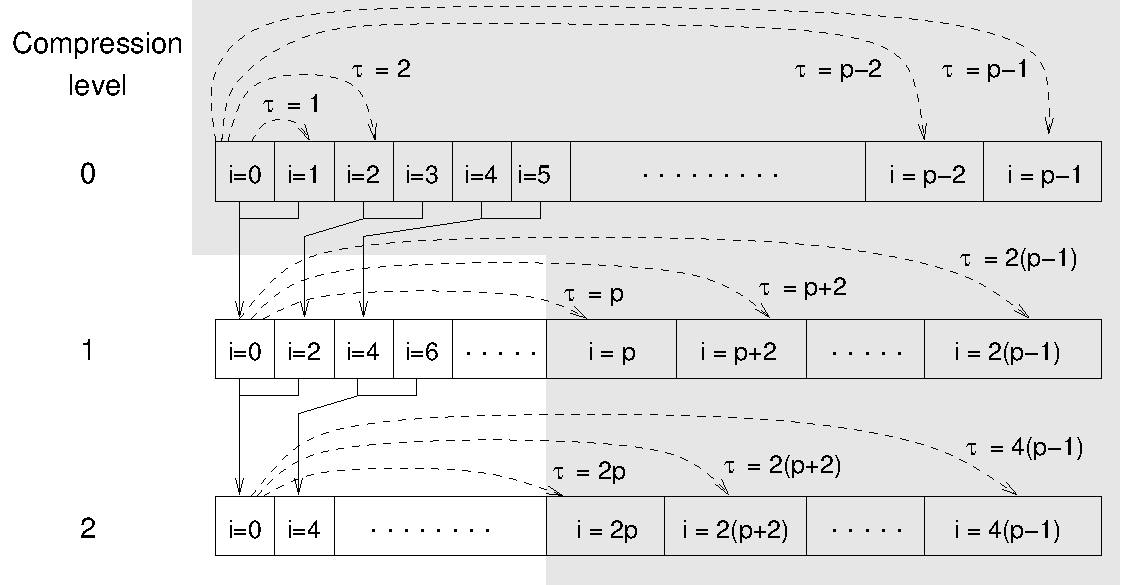
\includegraphics[width=0.9\textwidth]{figures/correlator_scheme}
\end{center} 
\caption{Schematic representation of buffers in the correlator.}
\label{fig:dataSet}
\end{figure}

Let us consider a set of $N$ observable values as schematically shown
in Figures~\ref{fig:dataSet}, where a value of index $i$ was measured
in time $i\delta t$. We are interested in computing the correlation 
function according to Equation~\ref{eq:CtauDef} for a range lag times
$\tau = (i-j)\delta t$ between the measurements $i$ and $j$.
To simplify the notation, we further drop $\delta t$
when refering to observables and lag times. 

The trivial implementation takes all possible pairs of values
corresponding to lag times $\tau \in [\taumin:\taumax]$. 
Without loss of generality, let us further consider $\taumin=0$.
The computational effort for such an algorithm scales
as ${\cal O} \bigl(\taumax^2\bigr)$.
As a rule of thumb, this is feasible if $\taumax < 10^3$.
The multiple tau correlator provides a solution to compute the
correlation functions for arbitrary range of the lag times by
coarse-graining the high $\tau$ values. It applies the naive algorithm
to a relatively small range of lag times $\tau \in [0:p-1]$. This we refer
to as compression level 0. To compute the correlations for lag times
$\tau \in [p:2(p-1)]$, the original data are first coarse-grained, so
that $m$ values of the original data are compressed to produce a single
data point in the higher compression level. Thus the lag time between
the neighbouring values in the higher compression level increases
by a factor of $m$, while the number of stored values decreases by
the same factor and the number of correlation operations at this level
reduces by a factor of $m^2$. Correlations for lag times 
$\tau \in [2p:4(p-1)]$ are computed at compression level 2, which is created
in an analogous manner from level 1. This can continue hierarchically
up to an arbitrary level for which enough data is available. Due to the
hierarchical reduction of the data, the algorithm scales as 
${\cal O} \bigl( p^2 \log(\taumax) \bigr)$. Thus an additional order
of magnitude in $\taumax$ costs just a constant extra effort.

The speedup is gained at the expense of statistical accuracy.
The loss of accuracy occurs at the compression step.
In principle one can use any value of $m$ and $p$ to tune the algorithm
performance. However, it turns out that using a high $m$ dilutes the
data at high $\tau$. Therefore $m=2$ is hardcoded in the \es correlator
and cannot be modified by user. The value of $p$ remains an adjustable
parameter which can be modified by user by setting \lit{tau_lin}
when defining a correlation. In genral, one should choose $p \gg m$
to avoid loss of statistical accuracy. Choosing $p=16$ seems to be
safe but it may depend on the properties of the analyzed
corerlation functions. A detailed analysis has been performed
in Ref.~\cite{ramirez10a}.

The choice of the compression function also influences the statistical
accuracy and can even lead to systematic errors. The default compression 
function is \lit{discard2} which discards the second fo the compressed 
values and pushes the first one to the higher level. This is robust and 
can be applied universally to any combination of observables and
correlation operation. On the other hand, it reduces the
statistical accuracy as the compression level increases.
In many cases, the \lit{average} compression operation
can be applied, which averages the two neighbouring values
and the average then enters the higher level, preserving
almost the full statistical accuracy of the original data. 
In general, if averaging can be safely used or not, depends on the 
properties of the difference
\begin{equation} 
\frac{1}{2} (A_i \otimes B_{i+p} + A_{i+1} \otimes B_{i+p+1} ) - 
\frac{1}{2} (A_i + A_{i+1} ) \otimes \frac{1}{2} (B_{i+p} +  B_{i+p+1})
\label{eq:difference}
\end{equation} 
For example in the case of velocity autocorrelation function, the
above-mentioned difference has a small value and a random sign, \ie\ 
different contributions cancel each other. On the other hand, in the
of the case of mean square displacmenent the difference is always positive,
resulting in a non-negligible systematic error. A more general
discussion is presented in Ref.~\cite{ramirez10a}.


\section{\lit{uwerr}: Computing statistical errors in time series}
\label{sec:uwerr}
\newescommand{uwerr}

\begin{essyntax}
  \variant{1} uwerr \var{data} \var{nrep} 
  \var{col} \opt{\var{s\_tau}} \opt{plot}

  \variant{2} uwerr \var{data} \var{nrep} 
  \var{f} \opt{\var{s\_tau} \opt{\var{f\_args}}} \opt{plot}
\end{essyntax}
Calculates the mean value, the error and the error of the error for an
arbitrary numerical time series according to \citet{wolff04a}.

\begin{arguments}
\item[\var{data}] is a matrix filled with the primary estimates
  $a_\alpha^{i,r}$ from $R\/$ replica with $N_1,N_2,\ldots,N_R$
  measurements each.

  \begin{displaymath}
    \var{data}=\left(
      \begin{array}
        {*{4}{c}} a_1^{1,1}&a_2^{1,1}&a_3^{1,1}&\cdots\\ 
        a_1^{2,1}&a_2^{2,1}&a_3^{2,1}&\cdots\\
        \vdots&\vdots&\vdots&\vdots\\
        a_1^{{N_1},1}&a_2^{{N_1},1}&a_3^{{N_1},1}&\cdots\\
        a_1^{1,2}&a_2^{1,2}&a_3^{1,2}&\cdots\\
        \vdots&\vdots&\vdots&\vdots\\
        a_1^{{N_R},R}&a_2^{{N_R},R}&a_3^{{N_R},R}&\cdots\\
      \end{array}
    \right)
  \end{displaymath}
\item[\var{nrep}] is a vector whose elements specify the length of the
  individual replica. 
  \begin{displaymath}
    nrep=\left(N_1,N_2,\ldots,N_R\right)
  \end{displaymath}
\item[\var{f}] is a user defined Tcl function returning a double with
  first argument a vector which has as many entries as data has
  columns. If \var{f} is given instead of the column, the
  corresponding derived quantity is analyzed.

\item[\var{f\_args}] are further arguments to \var{f}.

\item[\var{s\_tau}] is the estimate $S=\tau/\tau_{\textrm{int}}$ as
  explained in section (3.3) of \cite{wolff04a}. The default is 1.5
  and it is never taken larger than $\min_{r=1}^R{N_r}/2$.

\item[\opt{plot}] If plot is specified, you will get the plots of
  $\Gamma/\Gamma(0)$ and $\tau_{int}$ vs. $W$.  The data and gnuplot
  script is written to the current directory.
\end{arguments}


\minisec{Output format}

\begin{code}
  \var{mean} \var{error} \var{error\_of\_error} \var{act}
  \var{error\_of\_act} \opt{\var{Q}}
\end{code}

where \var{act} denotes the integrated autocorrelation time, and
\var{Q} denotes a \emph{quality measure}, \ie the probability to find
a $\chi^2$ fit of the replica estimates.

The function returns an error message if the windowing failed or if
the error in one of the replica is to large.

%%% Local Variables: 
%%% mode: latex
%%% TeX-master: "ug"
%%% End: 
